
\documentclass[10pt]{beamer}\usepackage[]{graphicx}\usepackage[]{xcolor}
% maxwidth is the original width if it is less than linewidth
% otherwise use linewidth (to make sure the graphics do not exceed the margin)
\makeatletter
\def\maxwidth{ %
  \ifdim\Gin@nat@width>\linewidth
    \linewidth
  \else
    \Gin@nat@width
  \fi
}
\makeatother

\definecolor{fgcolor}{rgb}{0.345, 0.345, 0.345}
\newcommand{\hlnum}[1]{\textcolor[rgb]{0.686,0.059,0.569}{#1}}%
\newcommand{\hlstr}[1]{\textcolor[rgb]{0.192,0.494,0.8}{#1}}%
\newcommand{\hlcom}[1]{\textcolor[rgb]{0.678,0.584,0.686}{\textit{#1}}}%
\newcommand{\hlopt}[1]{\textcolor[rgb]{0,0,0}{#1}}%
\newcommand{\hlstd}[1]{\textcolor[rgb]{0.345,0.345,0.345}{#1}}%
\newcommand{\hlkwa}[1]{\textcolor[rgb]{0.161,0.373,0.58}{\textbf{#1}}}%
\newcommand{\hlkwb}[1]{\textcolor[rgb]{0.69,0.353,0.396}{#1}}%
\newcommand{\hlkwc}[1]{\textcolor[rgb]{0.333,0.667,0.333}{#1}}%
\newcommand{\hlkwd}[1]{\textcolor[rgb]{0.737,0.353,0.396}{\textbf{#1}}}%
\let\hlipl\hlkwb

\usepackage{framed}
\makeatletter
\newenvironment{kframe}{%
 \def\at@end@of@kframe{}%
 \ifinner\ifhmode%
  \def\at@end@of@kframe{\end{minipage}}%
  \begin{minipage}{\columnwidth}%
 \fi\fi%
 \def\FrameCommand##1{\hskip\@totalleftmargin \hskip-\fboxsep
 \colorbox{shadecolor}{##1}\hskip-\fboxsep
     % There is no \\@totalrightmargin, so:
     \hskip-\linewidth \hskip-\@totalleftmargin \hskip\columnwidth}%
 \MakeFramed {\advance\hsize-\width
   \@totalleftmargin\z@ \linewidth\hsize
   \@setminipage}}%
 {\par\unskip\endMakeFramed%
 \at@end@of@kframe}
\makeatother

\definecolor{shadecolor}{rgb}{.97, .97, .97}
\definecolor{messagecolor}{rgb}{0, 0, 0}
\definecolor{warningcolor}{rgb}{1, 0, 1}
\definecolor{errorcolor}{rgb}{1, 0, 0}
\newenvironment{knitrout}{}{} % an empty environment to be redefined in TeX

\usepackage{alltt}

\usepackage{xcolor}
\usepackage{mathtools}
\usepackage{graphicx} 
\usepackage{amsmath}
\usepackage{listings}
\lstnewenvironment{rc}[1][]{\lstset{language=R}}{}

\graphicspath{{images/}}
\usepackage{tikz} 
\usetikzlibrary{arrows,calc,patterns,positioning,shapes,decorations.markings} 
\usetikzlibrary{decorations.pathmorphing} 

%\usetheme{default}
\mode<presentation>
{
	\usetheme{Singapore}
	\usecolortheme{crane}
	% or ...
	
	\setbeamercovered{transparent}
	% or whatever (possibly just delete it)
}

\title{Introduction to Structural Equation Modeling using lavaan}
\subtitle{Multigroup Models \& Measurement Invariance}
\author{R. M. Kuiper (and many others)}
\institute{Department of Methodology \& Statistics \\ Utrecht University}
\date{}

%------------------------------------------------------------------------------%
%\hypersetup{bookmarksopen=false}
\hypersetup{bookmarksdepth=-2}
\AtBeginSection[]
{
    \begin{frame}
        \frametitle{Table of Contents}
        \tableofcontents[currentsection] %subsectionstyle=hide] %, hidesubsections]
    \end{frame}
}
\IfFileExists{upquote.sty}{\usepackage{upquote}}{}
\begin{document}


%------------------------------------------------------------------------------%

\begin{frame}[t, plain]
  \titlepage
\end{frame}

%------------------------------------------------------------------------------%
%
\begin{frame}{Outline of this lecture}
\tableofcontents[hidesubsections]
\end{frame}

%-----------------------------------------------------------
% SECTION 3
%------------------------------------------------------------------------------%
% Slide 71
\section{Multi-group (MG) analysis}
%\subsection*{Theory}
%------------------------------------------------------------------------------%
%
% Slide 1
\begin{frame}{From one group to multiple groups}
\begin{itemize}
    \item EFA or CFA for single group:\\
    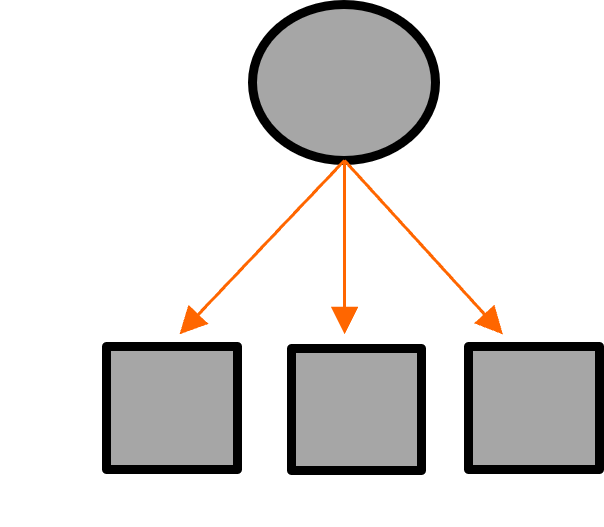
\includegraphics[height=3cm,keepaspectratio]{images/EFAandCFA.png} 
    \item EFA or CFA for multiple groups:\\
    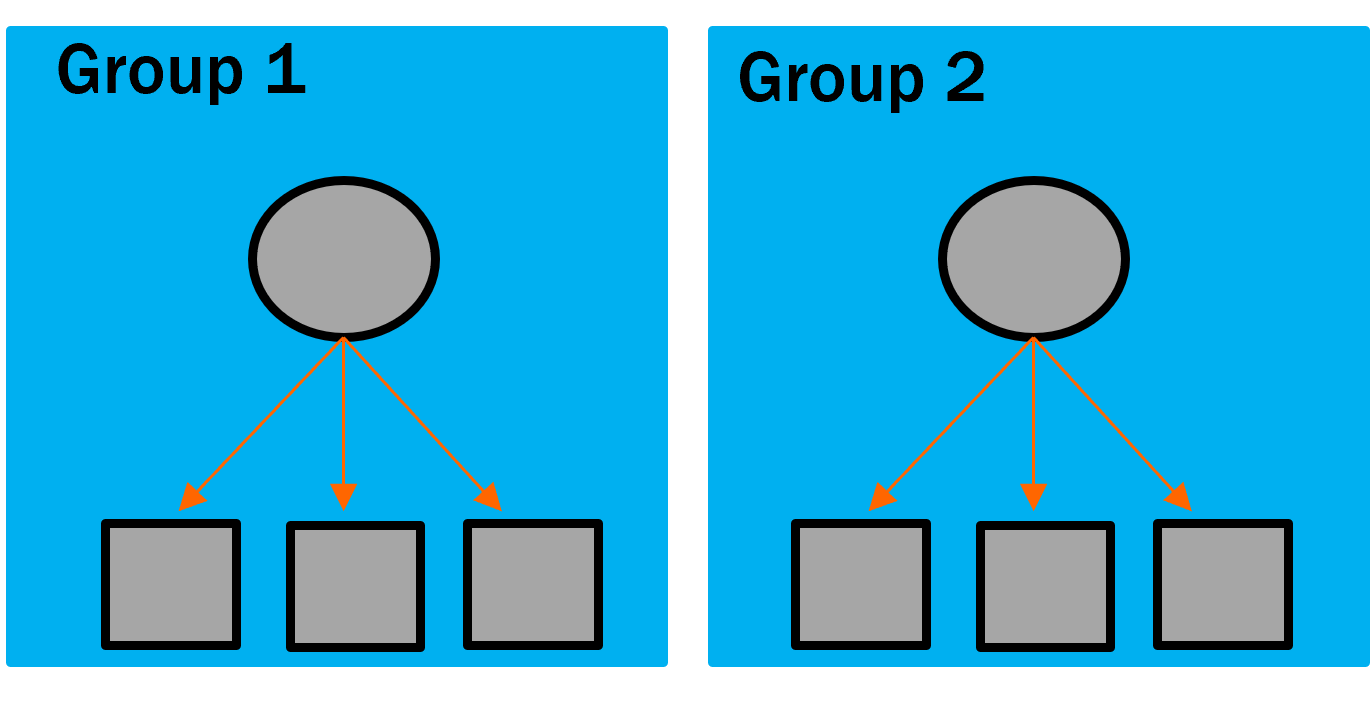
\includegraphics[height=3cm,keepaspectratio]{images/MultipleGroup.png} 
\end{itemize}
\end{frame}
%------------------------------------------------------------------------------%
%
%------------------------------------------------------------------------------%
%
% Slide 73-78
\begin{frame}{General setup of multigroup analysis}
    \begin{enumerate}
        \item Each group treated as \textbf{separate dataset}.
        \begin{itemize}
            \item  Like ``select data'' in SPSS: select people who meet a specific condition (e.g., female, Dutch, etc)
            \item lavaan does it behind the scenes, after denoting your groups.
        \end{itemize}
        \item Model is fitted in each group separately.
        \item Apply constraints to test whether parameters are the same / significantly different across different groups.
    \end{enumerate}
\end{frame}
%------------------------------------------------------------------------------%
%
%------------------------------------------------------------------------------%
\section{MG regression in R}
%------------------------------------------------------------------------------%
%
%------------------------------------------------------------------------------%
%
% Slide 72 + 79 
\begin{frame}{Example: Multigroup regression}

Regression example from lab meeting `Intro and regression':
\begin{itemize}
  \item{Outcome: sw}
  \item{Predictors: overt and covert}
  \item{Group: gender (males and females)}
\end{itemize}
          
\end{frame}
%------------------------------------------------------------------------------%
%
% Slide 79 + 80
\begin{frame}[fragile]{Multigroup regression - lavaan model}

\begin{knitrout}
\definecolor{shadecolor}{rgb}{0.969, 0.969, 0.969}\color{fgcolor}\begin{kframe}
\begin{alltt}
\hlcom{# Data}
\hlstd{data_regr} \hlkwb{<-} \hlkwd{read.table}\hlstd{(}\hlstr{"popular_regr.txt"}\hlstd{,} \hlkwc{header} \hlstd{= T)}
\hlstd{data_regr[}\hlkwd{sapply}\hlstd{(data_regr,} \hlkwa{function}\hlstd{(}\hlkwc{x}\hlstd{)}
          \hlkwd{as.character}\hlstd{(x)} \hlopt \hlkwd{c}\hlstd{(}\hlstr{"-99"}\hlstd{,} \hlstr{"-999"}\hlstd{) )]} \hlkwb{<-} \hlnum{NA}
\hlstd{data_regr}\hlopt{$}\hlstd{gender} \hlkwb{<-} \hlkwd{factor}\hlstd{(data_regr}\hlopt{$}\hlstd{gender,}
                           \hlkwc{labels} \hlstd{=} \hlkwd{c}\hlstd{(}\hlstr{"male"}\hlstd{,} \hlstr{"female"}\hlstd{))}

\hlcom{# Model}
\hlstd{model.MGregr} \hlkwb{<-} \hlstr{'
  sw ~ overt + covert # regression
  sw ~~ sw            # residual variance
  sw ~ 1              # intercept
'}
\end{alltt}
\end{kframe}
\end{knitrout}
          
\end{frame}
%------------------------------------------------------------------------------%
%
% Slide 79 + 80
\begin{frame}[fragile]{Multigroup regression - fit lavaan model}

Use the `group' argument in lavaan:

\vspace{5mm}

\begin{knitrout}
\definecolor{shadecolor}{rgb}{0.969, 0.969, 0.969}\color{fgcolor}\begin{kframe}
\begin{alltt}
\hlcom{# Fit model}
\hlstd{fit.MGregr} \hlkwb{<-} \hlkwd{lavaan}\hlstd{(model.MGregr,} \hlkwc{data} \hlstd{= data_regr,}
              \hlkwc{group} \hlstd{=} \hlstr{"gender"}\hlstd{)} \hlcom{# multigroup specification}
\end{alltt}


{\ttfamily\noindent\color{warningcolor}{\#\# Warning in lav\_data\_full(data = data, group = group, cluster = cluster, : lavaan WARNING: group variable 'gender' contains missing values}}\begin{alltt}
\hlcom{# Results}
\hlcom{#summary(fit.MGregr) # or:}
\hlcom{#summary(fit.MGregr, standardized = TRUE)}
\end{alltt}
\end{kframe}
\end{knitrout}
          
\end{frame}
%------------------------------------------------------------------------------%
%
% Slide 81
\begin{frame}[fragile]{Multigroup regression - lavaan output}

\footnotesize{
\begin{verbatim}
                   Estimate  Std.Err  z-value  P(>|z|)
Group 1 [male]:

Regressions:
  sw ~                                                
    overt            -0.278    0.059   -4.719    0.000
    covert           -0.497    0.039  -12.818    0.000
Intercepts:
   .sw                4.930    0.085   57.938    0.000
Variances:
   .sw                0.336    0.017   19.442    0.000

Group 2 [female]:

Regressions:
  sw ~                                                
    overt            -0.232    0.081   -2.871    0.004
    covert           -0.558    0.045  -12.295    0.000
Intercepts:
   .sw                5.062    0.106   47.703    0.000
Variances:
   .sw                0.318    0.019   17.044    0.000
\end{verbatim}    
}
\end{frame}
%------------------------------------------------------------------------------%
%
%\subsection*{Test}
%\section{Equality of coefficients test}
%------------------------------------------------------------------------------%
%
% Slide 83-85
\begin{frame}[fragile]{Multigroup regression: Test equality of coefficients}

\begin{knitrout}
\definecolor{shadecolor}{rgb}{0.969, 0.969, 0.969}\color{fgcolor}\begin{kframe}
\begin{alltt}
\hlcom{# Model specification}
\hlstd{model.MGregr_equal} \hlkwb{<-} \hlstr{'
  # model with labeled parameters
  sw ~ c(b1_m,b1_f)*overt + c(b2_m,b2_f)*covert 
  sw ~~ sw                                      
  sw ~ 1                                        
'}

\hlcom{# Fit model}
\hlstd{fit_MGregr_equal} \hlkwb{<-} \hlkwd{lavaan}\hlstd{(}\hlkwc{model} \hlstd{= model.MGregr_equal,}
                    \hlkwc{data} \hlstd{= data_regr,}
                    \hlkwc{group} \hlstd{=} \hlstr{"gender"}\hlstd{)} \hlcom{# multigroup specification }

\hlcom{# Test equality of regression coefficients}
\hlkwd{lavTestWald}\hlstd{(fit_MGregr_equal,}
            \hlkwc{constraints} \hlstd{=} \hlstr{'b1_m == b1_f; b2_m == b2_f'}\hlstd{)}
\end{alltt}
\end{kframe}
\end{knitrout}

\end{frame}


                    
  
%------------------------------------------------------------------------------%
%
% % Slide 87 - 89
% \begin{frame}{Multigroup regression: Output}
% 
% We use model fit to evaluate whether we can consider the coefficients equal across groups or not. \vspace{5mm}
% 
% Good fit of the model with constraints is not sufficient to conclude that the coefficients are equal across groups.\vspace{5mm}
% 
% We need to compare the fit of the model with constrained coefficients to thef it of the model with unconstrained coefficients.\vspace{5mm}
% 
% These models are nested (as was discussed yesterday), so we can use a chi-square difference test. \vspace{5mm}
% 
% \end{frame}
%------------------------------------------------------------------------------%
%
% Slide 90
\begin{frame}[fragile]{Comparing nested models}

Note: $constraints = 'b1_m == b1_f; b2_m == b2_f'$,\\
so comparison of two nested models.\\
Thus, one can perform a ${\chi}^2_\Delta$ test.

\vspace{5mm}

To compare fit of two nested models, you need:
\begin{enumerate}
    \item ${\chi}^2$ of the constrained model (${\chi}^2_C$)
    \item $df_C$ of the constrained model
    \item ${\chi}^2$ of the unconstrained model(${\chi}^2_U$)
    \item $df_U$ of the unconstrained model 
\end{enumerate}

Then, subtract: ${\chi}^2_C$ - ${\chi}^2_u$ = ${\chi}^2_\Delta$,\\
where ${\chi}^2_\Delta$ follows a Chi-square distribution with $df = df_C$-$df_U$. 

\vspace{5mm}

The function lavTestWald() does this for you!

\end{frame}
%------------------------------------------------------------------------------%
%
% Slide 91
\begin{frame}[fragile]{Comparing nested models Ctd.}

\textbf{Hypotheses} \\
$H_0$: Unconstrained model fit = constrained model fit \\
$H_A$: Unconstrained model fit $\neq$ constrained model fit

\vspace{5mm}

\textbf{High p-values:} No significant difference between the model fits: \\
No evidence that the coefficients differ across groups. 

\vspace{5mm}

\textbf{Low p-values:} Significant difference between the model fits: \\
Evidence that the coefficients differ across groups. 

\end{frame}
%------------------------------------------------------------------------------%
%
% Slide 92-93
\begin{frame}[fragile]{Multigroup regression: Test equality of coefficients Ctd.}

\footnotesize{
\begin{knitrout}
\definecolor{shadecolor}{rgb}{0.969, 0.969, 0.969}\color{fgcolor}\begin{kframe}
\begin{alltt}
\hlcom{# Test equality of regression coefficients \textbackslash{} Wald test}
\hlkwd{lavTestWald}\hlstd{(fit_MGregr_equal,}
            \hlkwc{constraints} \hlstd{=} \hlstr{'b1_m == b1_f; b2_m == b2_f'}\hlstd{)}
\end{alltt}
\begin{verbatim}
## $stat
## [1] 1.035524
## 
## $df
## [1] 2
## 
## $p.value
## [1] 0.5958526
## 
## $se
## [1] "standard"
\end{verbatim}
\begin{alltt}
\hlcom{# Could also specify both models and use anova()}
\end{alltt}
\end{kframe}
\end{knitrout}
}

Hence, $\Delta \chi^2 = 1.035, \chi^2(2) = 1.035, p=.596$.



\end{frame}
%------------------------------------------------------------------------------%
%
% Slide 94
\begin{frame}{Multigroup regression: Test conclusion}

Test result: $\chi^2(2) = 1.035, p=.596$.

\vspace{5mm}

Test conclusion:
\begin{itemize}
    \item No evidence for a difference in model fit for the constrained and the unconstrained models.
    \item No evidence for a difference in the regression coefficients.
    \item The overt coefficients are the same for males and females.
\end{itemize}

    
\end{frame}
%------------------------------------------------------------------------------%
%
% % Slide 95
% \begin{frame}{Multigroup regression: Test remarks}
% 
%     \begin{itemize}
%         \item We tested for both coefficients at once whether they differed across groups
%         \item It is also possible to test this for one coefficient at a time
%         \item For example, if our test for the coefficients at once was significant (there is a difference across groups), it would be an option to evaluate the coefficients separately as well. 
%         \item But: keep in mind issues with multiple testing. Doing a lot of tests means a lot of opportunity to make errors. 
%     \end{itemize}
%     
% \end{frame}
%------------------------------------------------------------------------------%
%
%------------------------------------------------------------------------------%
%-----------------------------------------------
% SECTION 3
\section{Measurement invariance (MI)}
%------------------------------------------------------------------------------%
%
%------------------------------------------------------------------------------%
%
% Slide 96
\begin{frame}{Measurement invariance}

Important in case of latent variables and multiple groups. 
    
\end{frame}
%------------------------------------------------------------------------------%
%
% Slide 97 - 103
\begin{frame}{Is my measurement model the same in different groups?}

\textbf{Construct validity:} \\
Is the model measuring the same thing for boys and girls? Or across different countries? 

\vspace{5mm}

\textbf{Can we make a fair comparison between groups?} \\
Did the groups understand the questions in the same way? 

\vspace{5mm}

\textbf{Same latent score should result in the same observed scores.}\\
We want (at least):
\begin{itemize}
    \item Equal intercepts (= item means)
    \item Equal slopes (factor loadings)
\end{itemize}

\end{frame}
%------------------------------------------------------------------------------%
%
% Slide 104-105
\begin{frame}{Stated differently}
    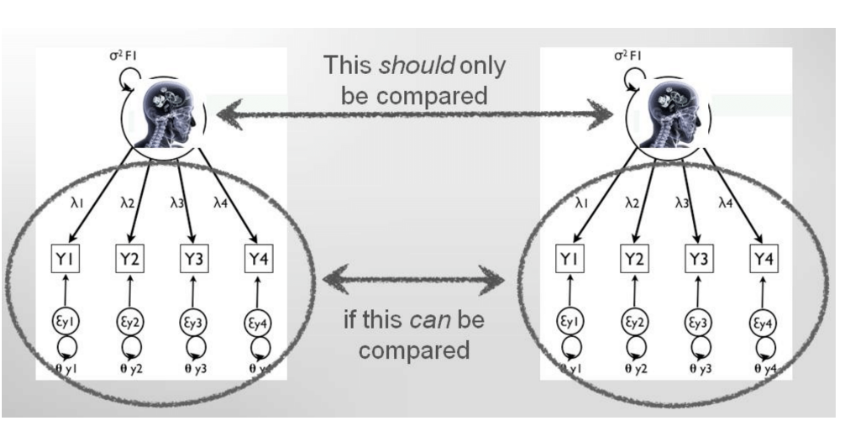
\includegraphics[width=\linewidth,height=\textheight,keepaspectratio]{images/slide105.png}
\end{frame}

% Slide 106
\begin{frame}{Stated differently...}
    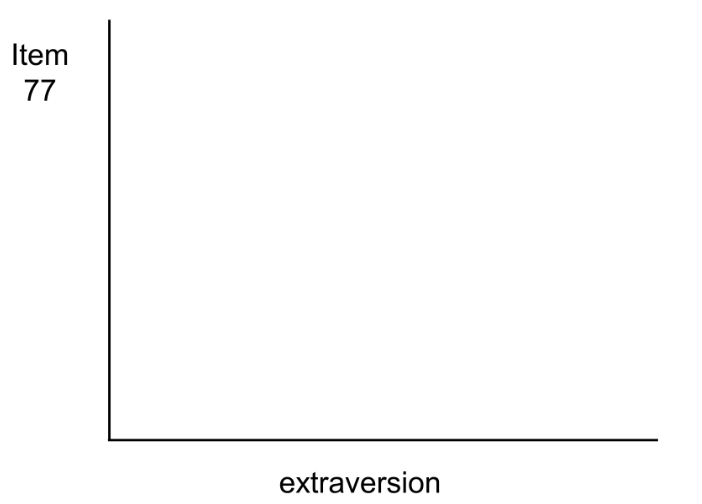
\includegraphics[height=0.8\textheight,keepaspectratio]{images/slide106.png}
\end{frame}

% Slide 107
\begin{frame}{Stated differently...}
    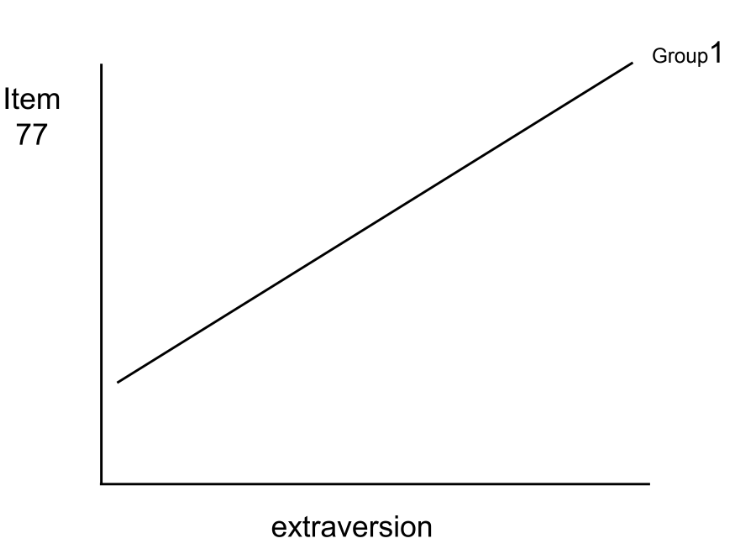
\includegraphics[height=0.8\textheight,keepaspectratio]{images/slide107.png}
\end{frame}

% Slide 108
\begin{frame}{Stated differently...}
    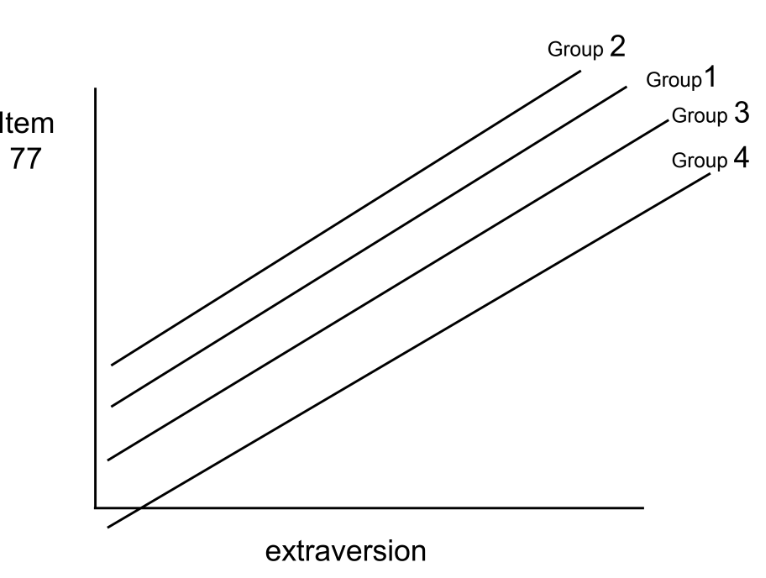
\includegraphics[height=0.8\textheight,keepaspectratio]{images/slide108.png}
\end{frame}

% Slide 109
\begin{frame}{Stated differently...}
    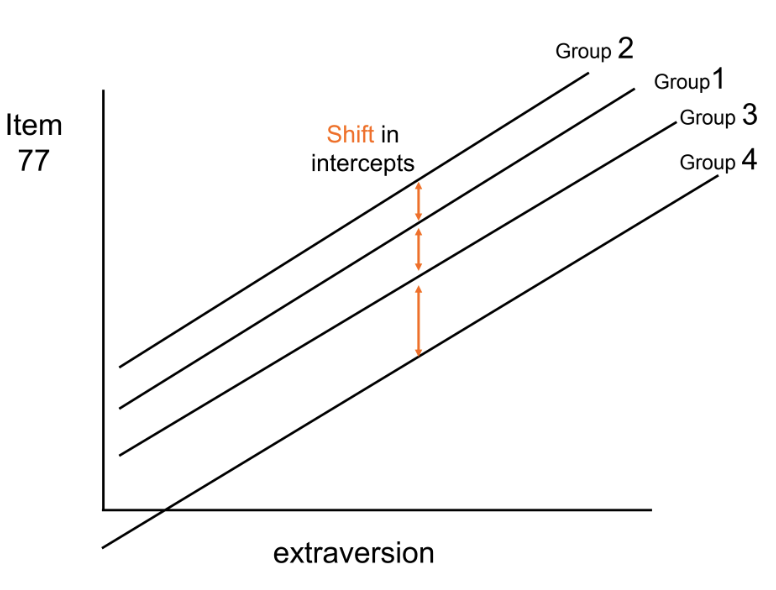
\includegraphics[height=0.8\textheight,keepaspectratio]{images/slide109.png}
\end{frame}

% Slide 110
\begin{frame}{Stated differently...}
    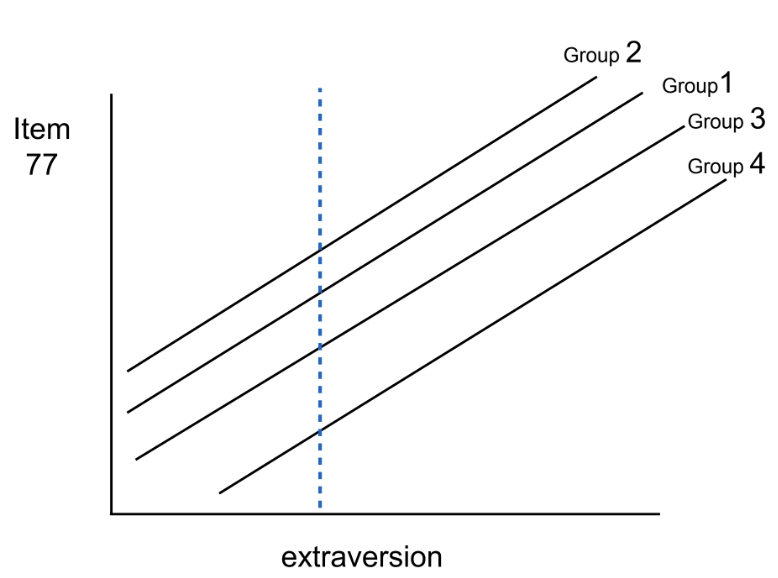
\includegraphics[height=0.8\textheight,keepaspectratio]{slide110.png}
\end{frame}

% Slide 111
\begin{frame}{Stated differently...}
    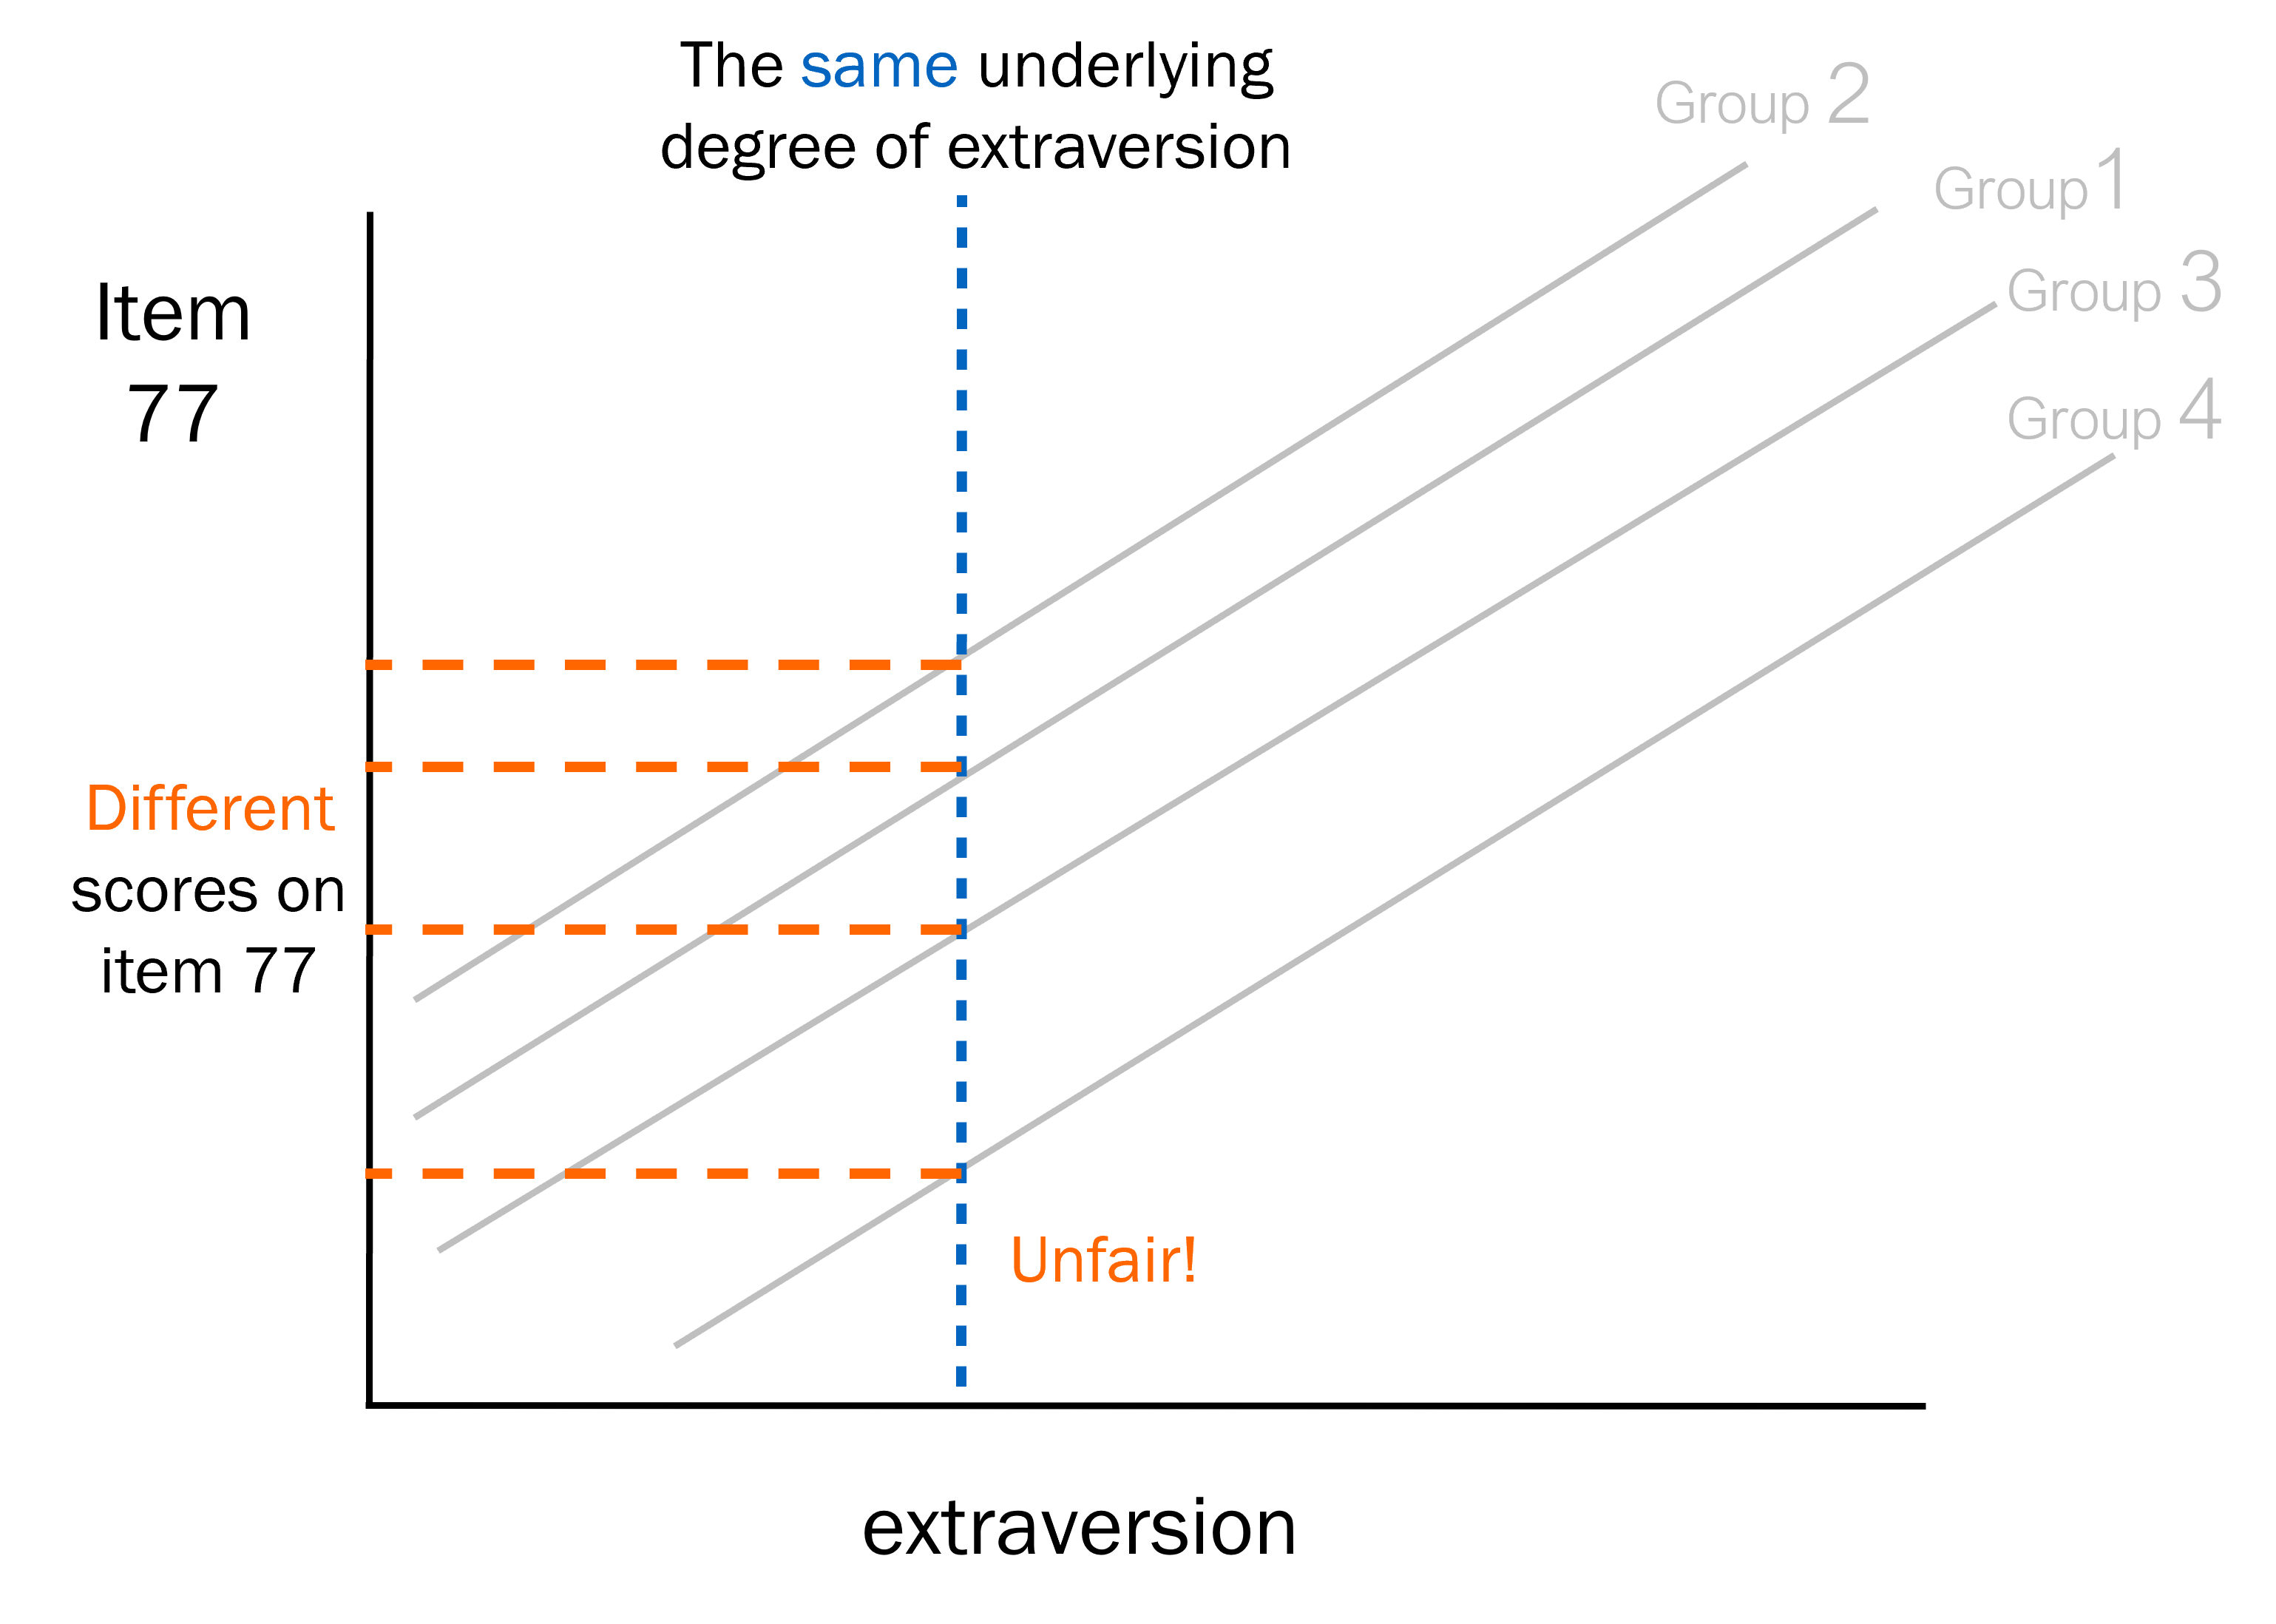
\includegraphics[height=0.8\textheight,keepaspectratio]{images/slide111.png}
\end{frame}

% Slide 112
\begin{frame}{Stated differently...}
    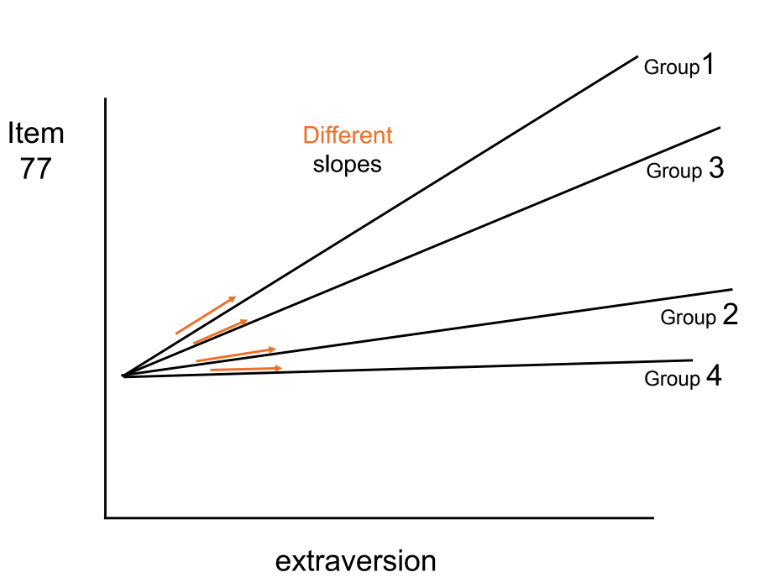
\includegraphics[height=0.8\textheight,keepaspectratio]{images/slide112.png}
\end{frame}

% Slide 113
\begin{frame}{Stated differently...}
    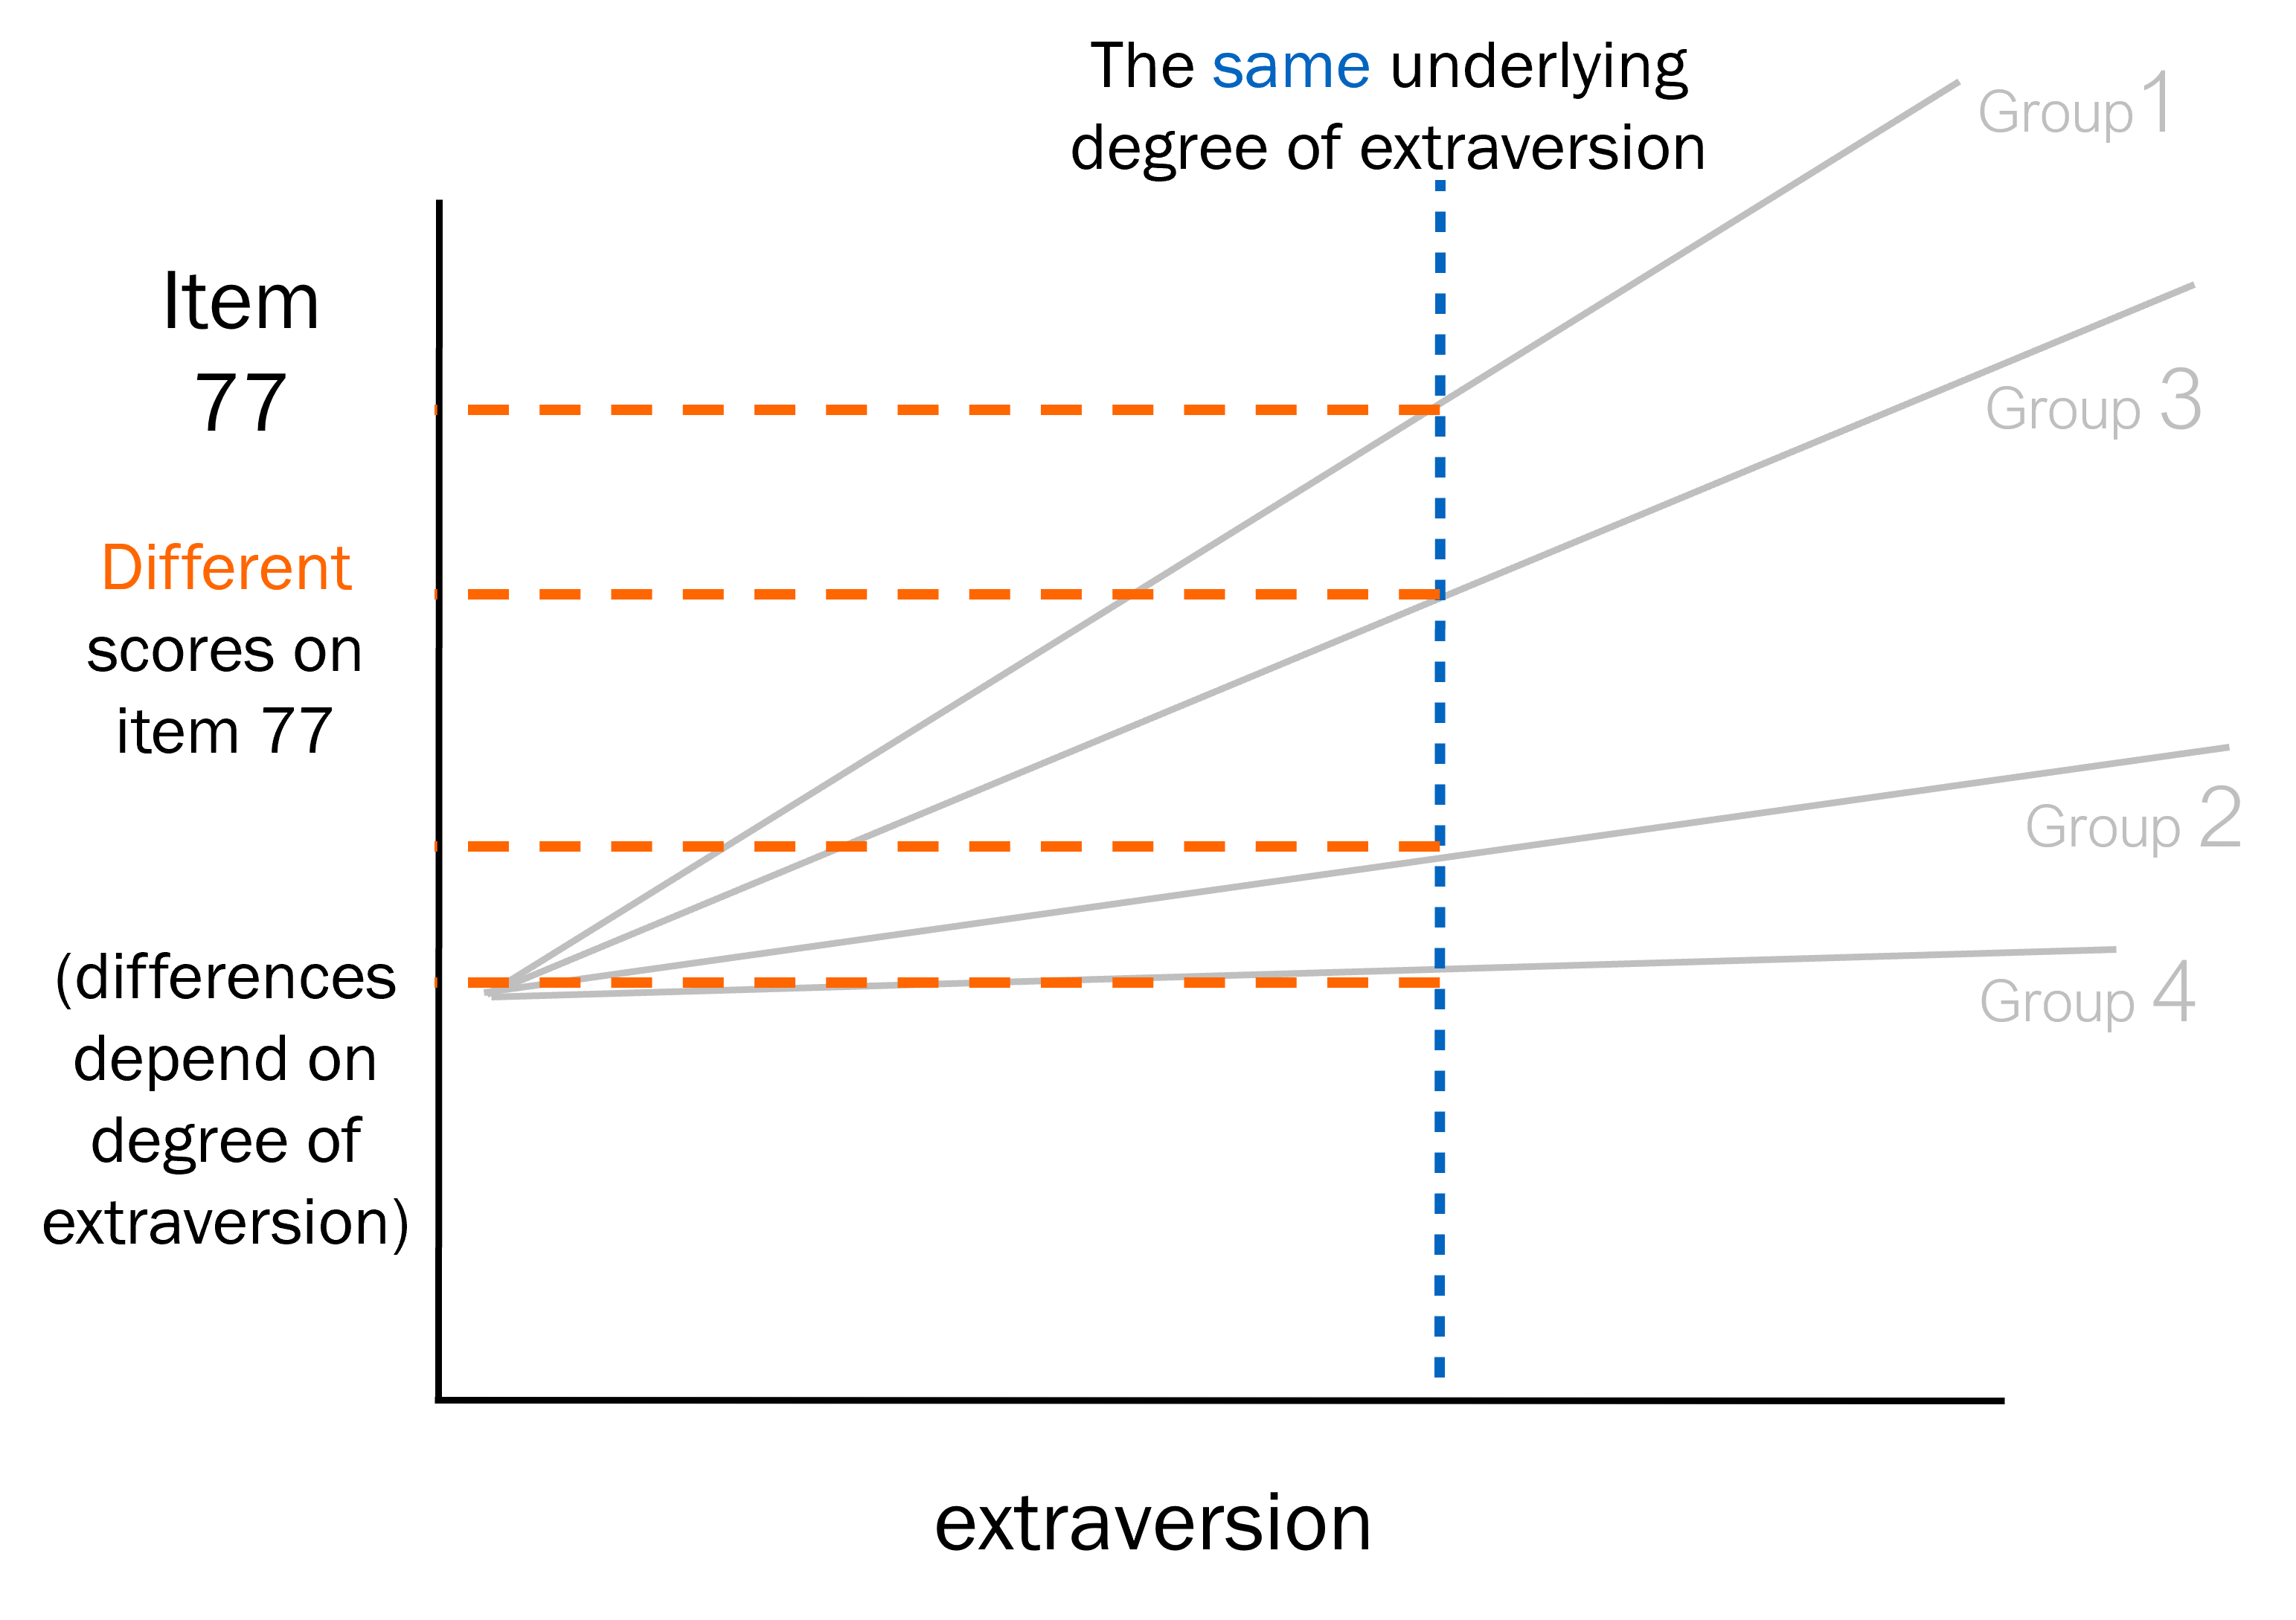
\includegraphics[height=0.8\textheight,keepaspectratio]{images/slide113.png}
\end{frame}

% Slide 114
\begin{frame}{Stated differently...}
    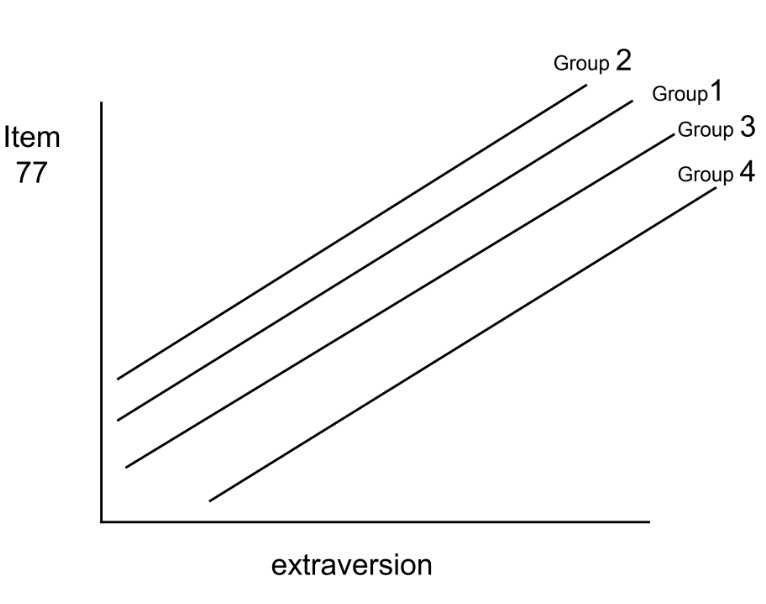
\includegraphics[height=0.8\textheight,keepaspectratio]{images/slide114.png}
\end{frame}

% Slide 115
\begin{frame}{Stated differently...}
    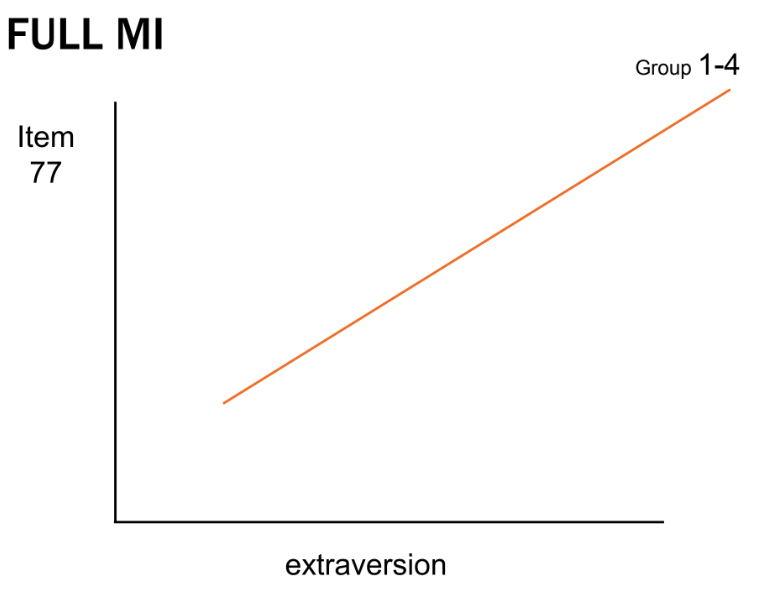
\includegraphics[height=0.8\textheight,keepaspectratio]{images/slide115.png}
\end{frame}

% Slide 116
\begin{frame}{Stated differently...}
    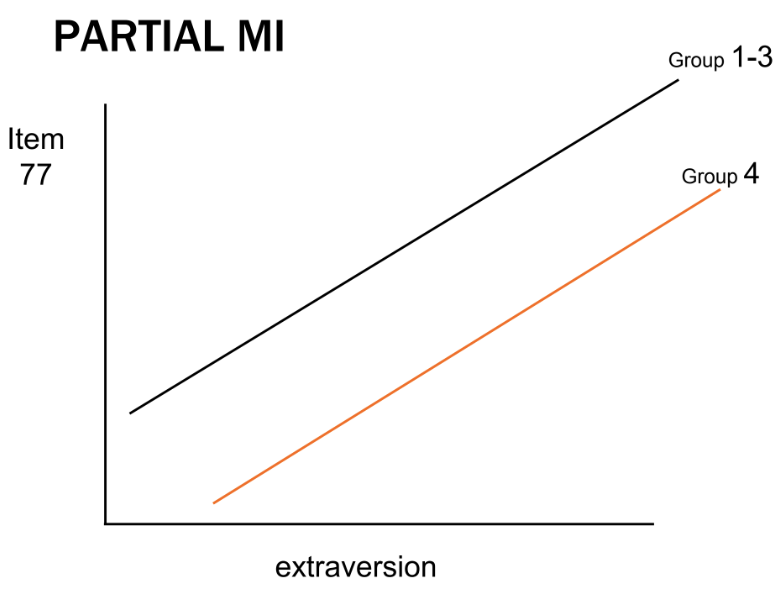
\includegraphics[height=0.8\textheight,keepaspectratio]{images/slide116.png}
\end{frame}
%------------------------------------------------------------------------------%
%
%\subsection*{MI - Part 2}
%------------------------------------------------------------------------------%
%
% Slide 117
\begin{frame}[fragile]{Measurement invariance}

\textbf{Exploratory approach:}
    \begin{itemize}
        \item Find a good factor structure.
        \item Impose constraints one-by-one.
    \end{itemize}
\vspace{5mm}
\textbf{Confirmatory approaches:}  
    \begin{enumerate}
        \item Bottom-up:
        \begin{itemize}
            \item Start with a CFA in each group separately.
            \item Impose equality constrained one by one. \\
            \textit{Note: multiple variations on the procedure possible.}
        \end{itemize}
        %\vspace{5mm}
        \item Top-down:
        \begin{itemize}
            \item Assume complete measurement invariance.
            \item Check in modification indices for constrains that if released would significantly improve the model.
        \end{itemize}
    \end{enumerate}
    
\end{frame}
%------------------------------------------------------------------------------%
%
% Slide 118
\begin{frame}[fragile]{Confirmatory bottom-up approach}

\textbf{Outline:}
    \begin{enumerate}
        \item Have the same factor structure across groups.\\
        No constraints, except same model structure.
        \item Have equal loadings across groups.
        \item Have equal intercepts across groups.
    \end{enumerate}
\vspace{5mm}
Equivalence is vital for valid comparisons across groups.\\
Partial equivalence may be acceptable. 
\end{frame}
%------------------------------------------------------------------------------%
%
% Slide 119
\begin{frame}[fragile]{Confirmatory bottom-up approach}
\begin{enumerate}
    \item Test overall model both groups combined.
    \item Test model separately for each group (\textbf{configural invariance}).
    \begin{itemize}
        \item Must fit the data
    \end{itemize}
    \item Test equality of loadings across groups (\textbf{metric/weak invariance}).
    \begin{itemize}
        \item Must be equal
    \end{itemize}
    \item Test equality of intercepts across groups (\textbf{scalar/strong invar.}).
    \begin{itemize}
        \item Must be equal
    \end{itemize}
    \item Test equality of measurement error variances (\textbf{strict invariance}).
    \begin{itemize}
        \item Not essential, often overly restrictive
    \end{itemize}
    \item Test equality of factor means / factor variances.
\end{enumerate}

\end{frame}
%------------------------------------------------------------------------------%
%
% Slide 121
\begin{frame}{Testing measurement invariance (MI)}

    \begin{columns}[T] % align columns
    \begin{column}{.75\textwidth}

        \begin{enumerate}
            \item Test overall model.
            \item Test model for groups separately.
            \item Test equal factor loadings ($\lambda_1$, $\lambda_2$, $\lambda_3$,).
            \item Test equal intercepts / item means ($\nu_1$, $\nu_2$, $\nu_3$,).
            \item Test equal residual/error variances ($\epsilon_1$, $\epsilon_2$, $\epsilon_3$,).
            \item Test factor means ($\alpha$) and/or variances ($\Psi$).
        \end{enumerate}
    \end{column}%

    \hfill%
    \begin{column}{.24\textwidth}

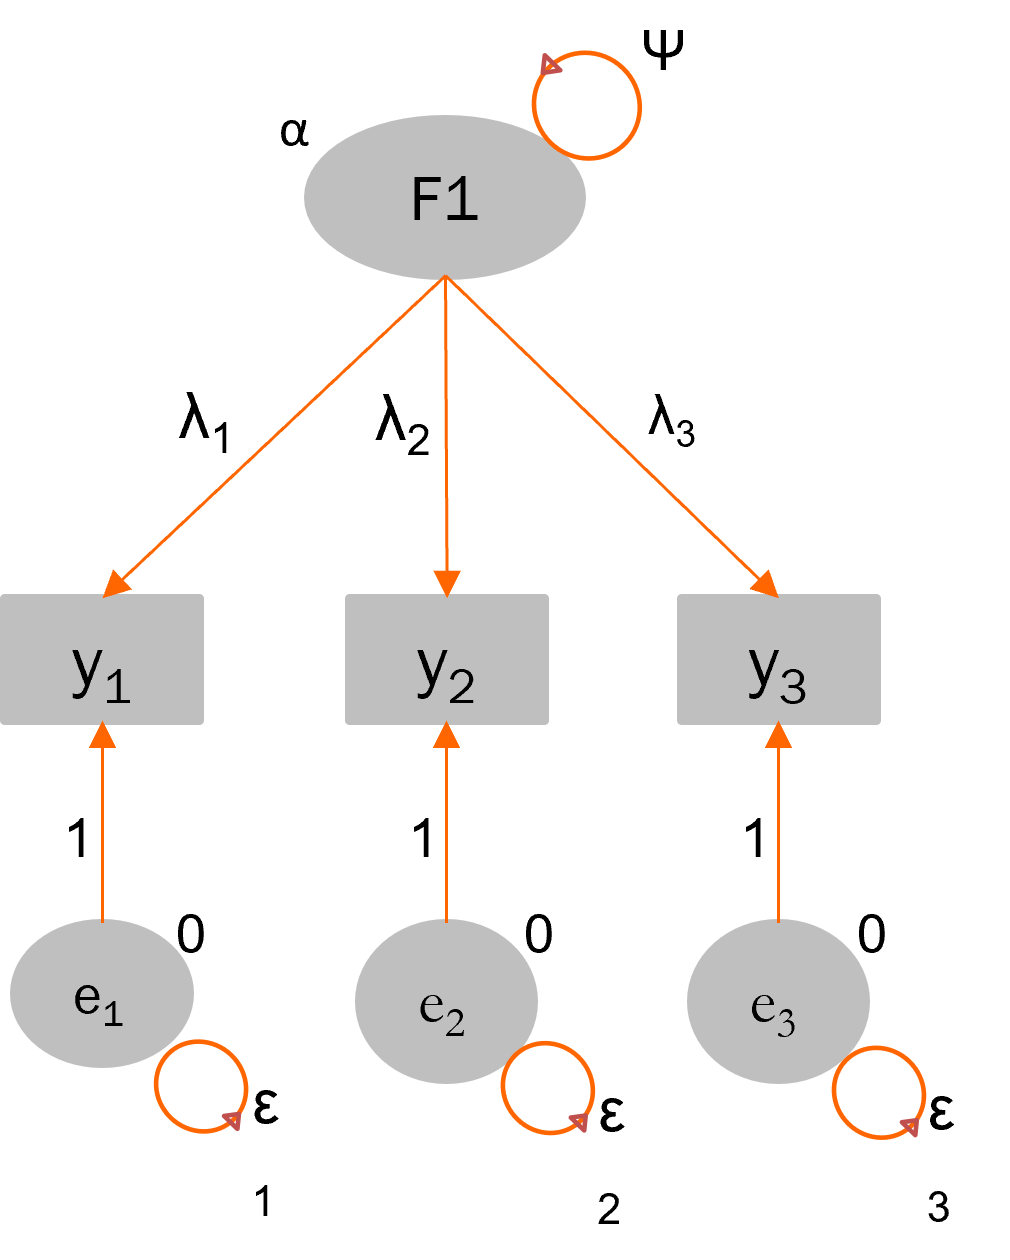
\includegraphics[width=\textwidth,keepaspectratio]{images/FactorModel.png}

    \end{column}%
    \end{columns}

\vspace{5mm}

Note: Steps 3, 4, and 5, that is, testing for configural invariance, metric/weak invariance, and scalar/strong invariance, respectively, are quite easily incorporated in lavaan.

\end{frame}
%------------------------------------------------------------------------------%
%
%------------------------------------------------------------------------------%
\section{MI in R}
%------------------------------------------------------------------------------%
%
%------------------------------------------------------------------------------%
% % Slide 120
% \begin{frame}
% 
%     \begin{center}
%     \Huge Measurement Invariance Example
%     \end{center}
% 
% \end{frame}
%------------------------------------------------------------------------------%
%
\begin{frame}{Example: South African Personality Inventory Project (SAPI)}
	
	
\includegraphics[height=7.5cm,keepaspectratio=T] {SAPI.png}
	
\end{frame}
%------------------------------------------------------------------------------%
%
\begin{frame}{CFA: only hypothesized loadings}
	
	\scalebox{0.6}{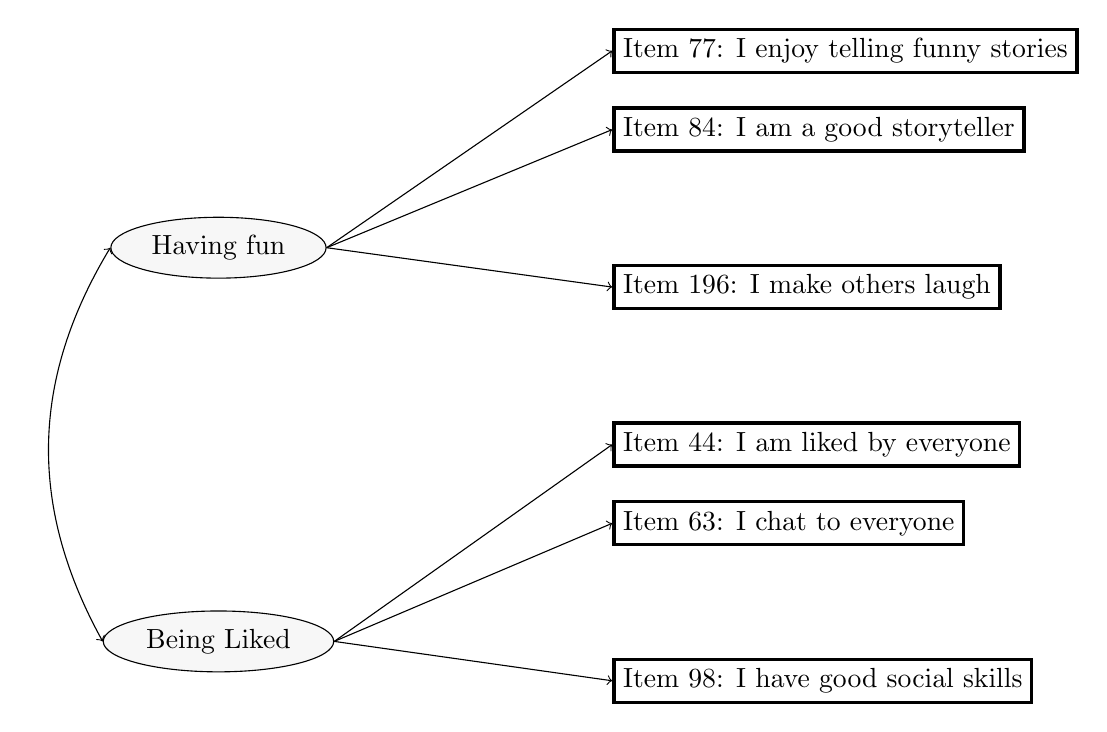
\begin{tikzpicture}[
			squarednode/.style={rectangle, draw=black, very thick, minimum size=5mm},
			arrow/.style = {thick}
			]
			\usetikzlibrary{shapes.geometric}
			
			%Nodes
			\node[ellipse, draw,fill=gray!6] at (-1,3) (latent) {Having fun};
			\node[squarednode,right=2cm of latent,yshift=0.5cm] at (2,5) (Item77) {Item 77: I enjoy telling funny stories}; 
			\node[squarednode,right=2cm of latent,yshift=0.5cm] at (2,4) (Item84) {Item 84: I am a good storyteller};
			\node[squarednode,right=2cm of latent,yshift=0.5cm] at (2,2) (Item196) {Item 196: I make others laugh};
			
			%%Arrows
			\draw[->] (latent.east) -- (Item77.west);
			\draw[->] (latent.east) -- (Item84.west);
			\draw[->] (latent.east) -- (Item196.west);
			
			%Nodes
			\node[ellipse, draw,fill=gray!6] at (-1,-2) (liked) {Being Liked};
			\node[squarednode,right=2cm of liked,yshift=0.5cm] at (2,0) (Item44) {Item 44: I am liked by everyone}; 
			\node[squarednode,right=2cm of liked,yshift=0.5cm] at (2,-1) (Item63) {Item 63: I chat to everyone};
			\node[squarednode,right=2cm of liked,yshift=0.5cm] at (2,-3) (Item98) {Item 98: I have good social skills};
			
			%%Arrows
			\draw[->] (liked.east) -- (Item44.west);
			\draw[->] (liked.east) -- (Item63.west);
			\draw[->] (liked.east) -- (Item98.west);
			
			\path[<->] (liked.west) edge [bend left] (latent.west);
			
	\end{tikzpicture}} 
	
	\vspace{5mm}
	
	In addition: group = 'Gender'
	
\end{frame}
%------------------------------------------------------------------------------%
%
% % Slide 122
% %\begin{frame}[fragile]{Testing measurement invariance in R: lavaan}
% \begin{frame}[fragile]{Testing measurement invariance with lavaan}
% 
% <<include=FALSE>>=
% # multigroup one-factor CFA (MG1CFA)
% model.1CFA <- '
%  factor1  =~ item1 + item2 + ...
% '
% 
% # configural invariance
% fit_MG1CFA_ci <- cfa(model.1CFA, data=data,
%                      group = 'group',
%                      missing='fiml', fixed.x=F)
% 
% # metric/weak invariance
% fit_MG1CFA_wi <- cfa(model.1CFA, data=data,
%                      group = 'group',
%                      missing='fiml', fixed.x=F,
%                      group.equal = "loadings")
% 
% # scalar/strong invariance
% fit_MG1CFA_si <- cfa(model.1CFA, data=data,
%                      group = 'group',
%                      missing='fiml', fixed.x=F,
%                      group.equal = c("intercepts", "loadings"))
% 
% # model comparison tests: anova() or lavTestLRT()
% lavTestLRT(fit_MG1CFA_ci, fit_MG1CFA_wi, fit_MG1CFA_si)
% @ 
% 
% \end{frame}
% %------------------------------------------------------------------------------%
% %
% % Slide 122
% \begin{frame}[fragile]{Testing measurement invariance in R: SEMtools}
% 
% % Does not exist anymore
% 
% <<include=FALSE>>=
% # multigroup one-factor CFA
% model.1CFA <- "
%  factor1  =~ item1 + item2 + ...
% "
% 
% # configural invariance
% # metric/weak invariance
% # scalar/strong invariance
% if (!require("semTools")) install.packages("semTools", dependencies = TRUE)
% library(semTools)
% measurementInvariance(model.1CFA, data=data,
%                       group = 'group',
%                       missing='fiml', fixed.x=F)
% @ 
% 
% \end{frame}
%------------------------------------------------------------------------------%
%
%------------------------------------------------------------------------------%
%
% Slide 122
\begin{frame}[fragile]{SAPI Example: MI models with lavaan}

\begin{knitrout}
\definecolor{shadecolor}{rgb}{0.969, 0.969, 0.969}\color{fgcolor}\begin{kframe}
\begin{alltt}
\hlcom{# Data}
\hlstd{data_sapi} \hlkwb{<-} \hlkwd{read.table}\hlstd{(}\hlstr{"Sapi.txt"}\hlstd{,} \hlkwc{header} \hlstd{= T)}

\hlstd{data_sapi[}\hlkwd{sapply}\hlstd{(data_sapi,}
    \hlkwa{function}\hlstd{(}\hlkwc{x}\hlstd{)} \hlkwd{as.character}\hlstd{(x)} \hlopt \hlkwd{c}\hlstd{(}\hlstr{"-999"}\hlstd{) )]} \hlkwb{<-} \hlnum{NA}

\hlstd{data_sapi}\hlopt{$}\hlstd{Gender} \hlkwb{<-} \hlkwd{factor}\hlstd{(data_sapi}\hlopt{$}\hlstd{Gender,} \hlkwc{labels} \hlstd{=} \hlkwd{c}\hlstd{(}\hlstr{"male"}\hlstd{,} \hlstr{"female"}\hlstd{))}
\end{alltt}
\end{kframe}
\end{knitrout}

\begin{knitrout}
\definecolor{shadecolor}{rgb}{0.969, 0.969, 0.969}\color{fgcolor}\begin{kframe}
\begin{alltt}
\hlcom{# multigroup two-factor CFA (MG2CFA) - group = 'Gender'}
\hlstd{model.2CFA} \hlkwb{<-} \hlstr{'
 Having fun  =~ Q77 + Q84 + Q196 
 Being liked =~ Q44 + Q63 + Q98
'}
\end{alltt}
\end{kframe}
\end{knitrout}

\end{frame}
%------------------------------------------------------------------------------%
%
\begin{frame}[fragile]{SAPI Example: MI models with lavaan Ctd.}

\begin{knitrout}
\definecolor{shadecolor}{rgb}{0.969, 0.969, 0.969}\color{fgcolor}\begin{kframe}
\begin{alltt}
\hlcom{# configural invariance}
\hlstd{fit_MG2CFA_ci} \hlkwb{<-} \hlkwd{cfa}\hlstd{(model.2CFA,} \hlkwc{data}\hlstd{=data_sapi,}
                     \hlkwc{group} \hlstd{=} \hlstr{'Gender'}\hlstd{,}
                     \hlkwc{missing}\hlstd{=}\hlstr{'fiml'}\hlstd{,} \hlkwc{fixed.x}\hlstd{=F)}

\hlcom{# metric/weak invariance}
\hlstd{fit_MG2CFA_wi} \hlkwb{<-} \hlkwd{cfa}\hlstd{(model.2CFA,} \hlkwc{data}\hlstd{=data_sapi,}
                     \hlkwc{group} \hlstd{=} \hlstr{'Gender'}\hlstd{,}
                     \hlkwc{missing}\hlstd{=}\hlstr{'fiml'}\hlstd{,} \hlkwc{fixed.x}\hlstd{=F,}
                     \hlkwc{group.equal} \hlstd{=} \hlstr{"loadings"}\hlstd{)}

\hlcom{# scalar/strong invariance}
\hlstd{fit_MG2CFA_si} \hlkwb{<-} \hlkwd{cfa}\hlstd{(model.2CFA,} \hlkwc{data}\hlstd{=data_sapi,}
                     \hlkwc{group} \hlstd{=} \hlstr{'Gender'}\hlstd{,}
                     \hlkwc{missing}\hlstd{=}\hlstr{'fiml'}\hlstd{,} \hlkwc{fixed.x}\hlstd{=F,}
                     \hlkwc{group.equal} \hlstd{=} \hlkwd{c}\hlstd{(}\hlstr{"intercepts"}\hlstd{,}
                                     \hlstr{"loadings"}\hlstd{))}
\end{alltt}
\end{kframe}
\end{knitrout}

\end{frame}
%------------------------------------------------------------------------------%
%
% Slide 123
\begin{frame}[fragile]{SAPI Example: Testing MI with lavaan}

\begin{knitrout}
\definecolor{shadecolor}{rgb}{0.969, 0.969, 0.969}\color{fgcolor}\begin{kframe}
\begin{alltt}
\hlcom{# model comparison tests: anova() or lavTestLRT()}
\hlkwd{lavTestLRT}\hlstd{(fit_MG2CFA_ci, fit_MG2CFA_wi,}
           \hlstd{fit_MG2CFA_si)[}\hlopt{-}\hlkwd{c}\hlstd{(}\hlnum{2}\hlstd{,}\hlnum{3}\hlstd{,}\hlnum{4}\hlstd{)]}
\end{alltt}
\begin{verbatim}
##               Df Chisq diff Df diff Pr(>Chisq)
## fit_MG2CFA_ci 16                              
## fit_MG2CFA_wi 20     1.3992       4     0.8443
## fit_MG2CFA_si 24     7.3791       4     0.1172
\end{verbatim}
\end{kframe}
\end{knitrout}

\begin{itemize}
    \item Metric/Weak invariance model fits just as well as the configural invariance model ($\chi^2(4) = 1.40$, $p = .84$).
    \item Scalar/Strong invariance model also fits just as well as the metric/weak invariance model ($\chi^2(4) = 7.38$, $p = .12$).
\end{itemize}

\end{frame}
%------------------------------------------------------------------------------%
%
% Slide 124
\begin{frame}{Testing MI with lavaan: IF significant}

\begin{itemize}
\item If the test for configural invariance against weak invariance is significant, then there is a lack of metric invariance and, thus, there is no need to test for scalar and strict invariance.\\
	\vspace{5mm}
    \item If tests significant: may try to find source of bias with modification indices.
    \item Then, aim for partial MI: Continue with MI tests with source of bias freely estimated between groups.
\end{itemize}

\end{frame}
%------------------------------------------------------------------------------%
%
% Slide 125-126
\begin{frame}[fragile]{SAPI Example: MI - Model comparison}

\begin{knitrout}
\definecolor{shadecolor}{rgb}{0.969, 0.969, 0.969}\color{fgcolor}\begin{kframe}
\begin{alltt}
\hlcom{# model comparison tests: anova() or lavTestLRT()}
\hlkwd{lavTestLRT}\hlstd{(fit_MG2CFA_ci, fit_MG2CFA_wi,}
           \hlstd{fit_MG2CFA_si)[}\hlkwd{c}\hlstd{(}\hlnum{2}\hlstd{,}\hlnum{3}\hlstd{)]}
\end{alltt}
\begin{verbatim}
##                 AIC   BIC
## fit_MG2CFA_ci 15354 15540
## fit_MG2CFA_wi 15348 15514
## fit_MG2CFA_si 15347 15494
\end{verbatim}
\end{kframe}
\end{knitrout}

\begin{itemize}
    \item Scalar/Strong invariance model fits best (lowest IC).
\end{itemize}

\end{frame}
%------------------------------------------------------------------------------%
%
% Slide 127
\begin{frame}[fragile]{SAPI Example: MI - Model fit}

\begin{knitrout}
\definecolor{shadecolor}{rgb}{0.969, 0.969, 0.969}\color{fgcolor}\begin{kframe}
\begin{alltt}
\hlcom{# model comparison tests: anova() or lavTestLRT()}
\hlstd{fitMI} \hlkwb{<-} \hlkwd{sapply}\hlstd{(}\hlkwd{list}\hlstd{(fit_MG2CFA_ci, fit_MG2CFA_wi,}
                     \hlstd{fit_MG2CFA_si),}
                \hlstd{fitMeasures,} \hlkwd{c}\hlstd{(}\hlstr{"cfi"}\hlstd{,} \hlstr{"rmsea"}\hlstd{))}
\hlkwd{colnames}\hlstd{(fitMI)} \hlkwb{<-} \hlkwd{c}\hlstd{(}\hlstr{"config"}\hlstd{,} \hlstr{"weak"}\hlstd{,} \hlstr{"strong"}\hlstd{)}
\hlstd{fitMI}
\end{alltt}
\begin{verbatim}
##           config       weak     strong
## cfi   0.93940080 0.94168219 0.93871806
## rmsea 0.09382256 0.08232267 0.07703613
\end{verbatim}
\begin{alltt}
\hlcom{# and many more measures...}
\end{alltt}
\end{kframe}
\end{knitrout}

\footnotesize{
$-$ Cheung, G. W., \& Rensvold, R. B. (2002). Evaluating goodness-of-fit indexes for testing measurement invariance. Structural Equation Modeling, 9(2), 233–255. doi:10.1207/S15328007SEM0902\_5

%\vspace{5mm}

$-$ Chen, F. F. (2007). Sensitivity of goodness of fit indexes to lack of measurement invariance. Structural Equation Modeling, 14(3), 464–504. doi:10.1080/10705510701301834
}
\end{frame}
%------------------------------------------------------------------------------%
%
% Slide 128
\begin{frame}{Further Reading}

Van de Schoot, R., Lugtig, P., \& Hox. J. (2012). A checklist for testing measurement invariance. European Journal of Developmental Psychology, 9,486-492. 

\vspace{5mm}

Vandenberg, R.J., \& Lance, C.E. (2000). A review and synthesis of the measurement invariance literature: Suggestions, practices, and recommendations for organizational research, Organizational Research Methods, 3, 4-70. 

\vspace{5mm}

Byrne, B.M., Shavelson, R.J., \& Muthén, B.O. (1989). Testing for equivalence of factor covariance and mean structures: The issue of partial measurement invariance. Psychological Bulletin, 105, 456-466. 

\vspace{5mm}

\textbf{Foundational Work:} Jöreskog, K.G. (1971). Simultaneous factor analysis in several populations. Psychometrika, 36, 409-426.

\end{frame}
%------------------------------------------------------------------------------%
%
% Slide 129 - Not
%
% Slide 130
\begin{frame}[fragile]{More interesting reading}
$-$ Van De Schoot, R., Kluytmans, A., Tummers, L., Lugtig, P., Hox, J., \& Muthén, B. (2013). Facing off with Scyllaand Charybdis:  A comparison of scalar, partial, and the novel possibility of approximate measurement invariance. Frontiers inPsychology, 4. 

%\vspace{5mm}

$-$ Fox, J.-P., \& Verhagen, A. J. (2010). Random item effects modeling for cross-national survey data.

%\vspace{5mm}

$-$ Davidov, P. Schmidt, \& J.Billiet (Eds.). Cross-cultural analysis: Methods and applications (pp. 467-488). London, UK: Routledge Academic. 

%\vspace{5mm}

$-$ Davidov, E., Dülmer, H., Schlüter, E., Schmidt, P., \& Meuleman, B. (2012). Using a multilevel structural equation modeling approach to explain cross cultural measurement noninvariance. Journal of Cross-Cultural Psychology, 43(4), 558–575. 

%\vspace{5mm}

$-$ Muthén, B., and Asparouhov, T.(2013). BSEM Measurement Invariance Analysis.  Mplus Web Notes: No. 17. 

%\vspace{5mm}

$-$ www.statmodel.com

\end{frame}
%------------------------------------------------------------------------------%
%
%------------------------------------------------------------------------------%
\section{The end}
%------------------------------------------------------------------------------%
%
%------------------------------------------------------------------------------%
%
\begin{frame}{Summary}

  \begin{itemize}
      \item Multi-group analysis
      \item Multi-group regression in R using lavaan
      \item Measurement invariance
      \item Measurement invariance in R using lavaan
  \end{itemize}

\end{frame}
% %------------------------------------------------------------------------------%
% %
% \begin{frame}{Take home message}
% \begin{itemize}
% \item{} 
%   \begin{itemize}
%   \item{}
%   \item{}
%   \end{itemize}
% \item{}
% \end{itemize}
% \end{frame}
%------------------------------------------------------------------------------%
%
\begin{frame}{Thanks \& How to proceed}

Thanks for listening!

\vspace*{5mm}

Are there any questions?\\
\begin{itemize}
  \item Ask fellow participant on course platform.
  \item Ask teacher during Q\&A (or via course platform).
  \item See if making the lab exercises help.
  \item Check the lavaan tutorial: e.g., \url{https://lavaan.ugent.be/tutorial/index.html}.
  \item Do not forget that Google is your best friend :-).
\end{itemize}

\vspace*{5mm}

You can start working on the lab exercises.

\end{frame}
%------------------------------------------------------------------------------%
%
%------------------------------------------------------------------------------%
%
\end{document}









